\begin{figbox}{!ht}
\caption{Dealing with unfair treatment}
\label{fig:treated1}

\sffamily
\footnotesize
\RaggedRight

\begin{tabular}{p{3.3cm} !{\quad} p{11cm}}
\addlinespace 
If I felt unfairly treated, I could feel comfortable reporting it.&
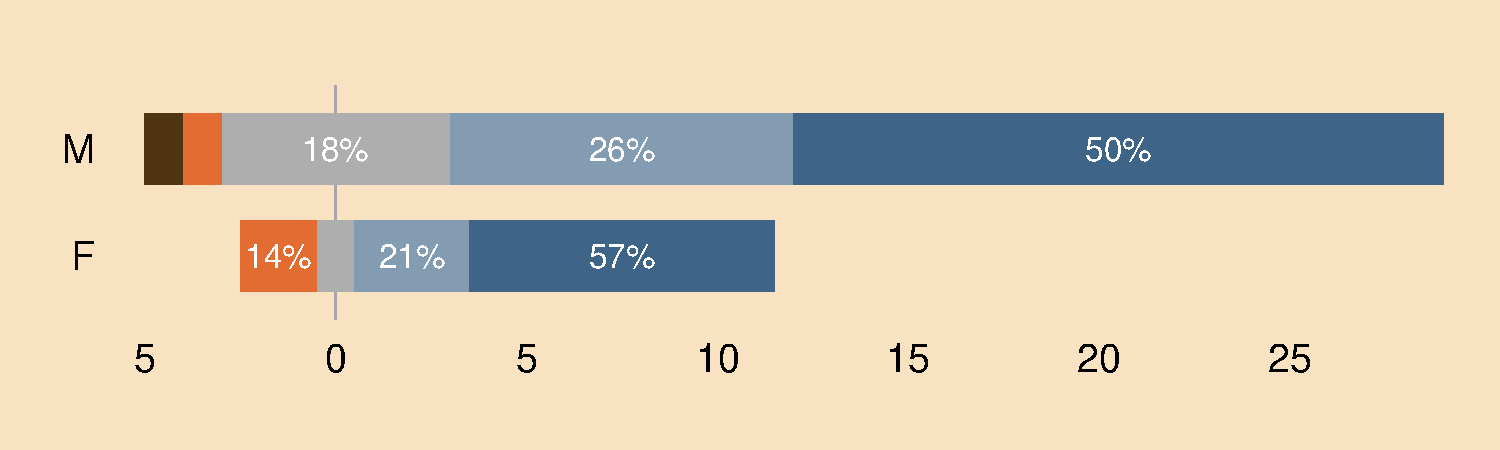
\includegraphics[align=t,trim={0 0 0 15mm},clip,width=11cm]{fig/culture/paolo1.pdf}\\

\hdashline

If I felt unfairly treated, I could identify a safe person to report this to & 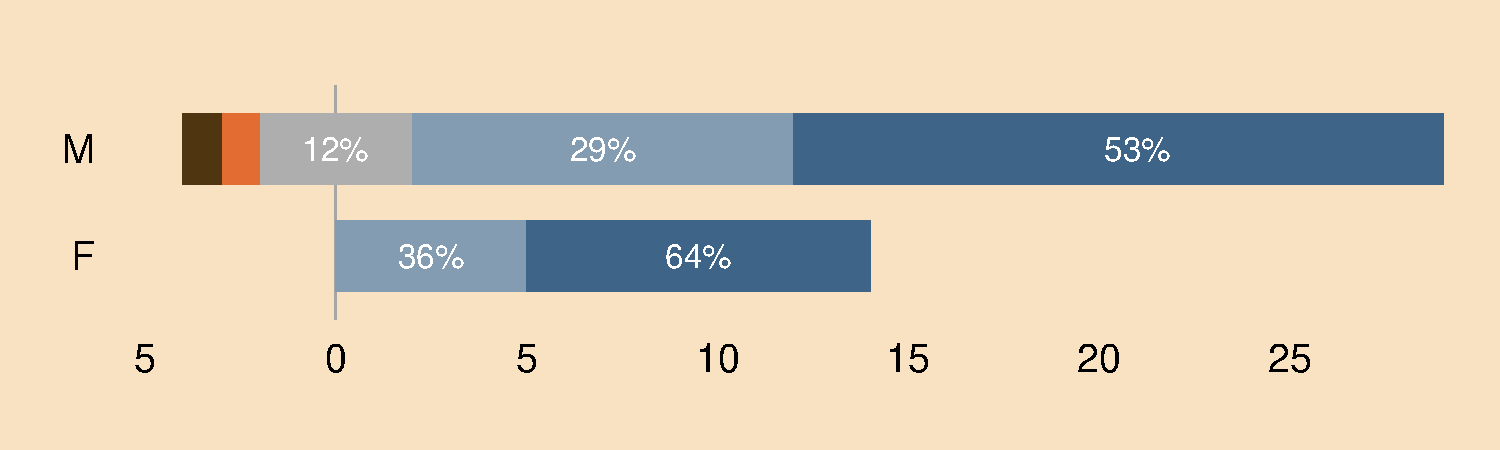
\includegraphics[align=t,trim={0 0 0 15mm},clip,width=11cm]{fig/culture/paolo2.pdf}\\

\hdashline
If I witnessed others treated unfairly, I would feel comfortable reporting it & 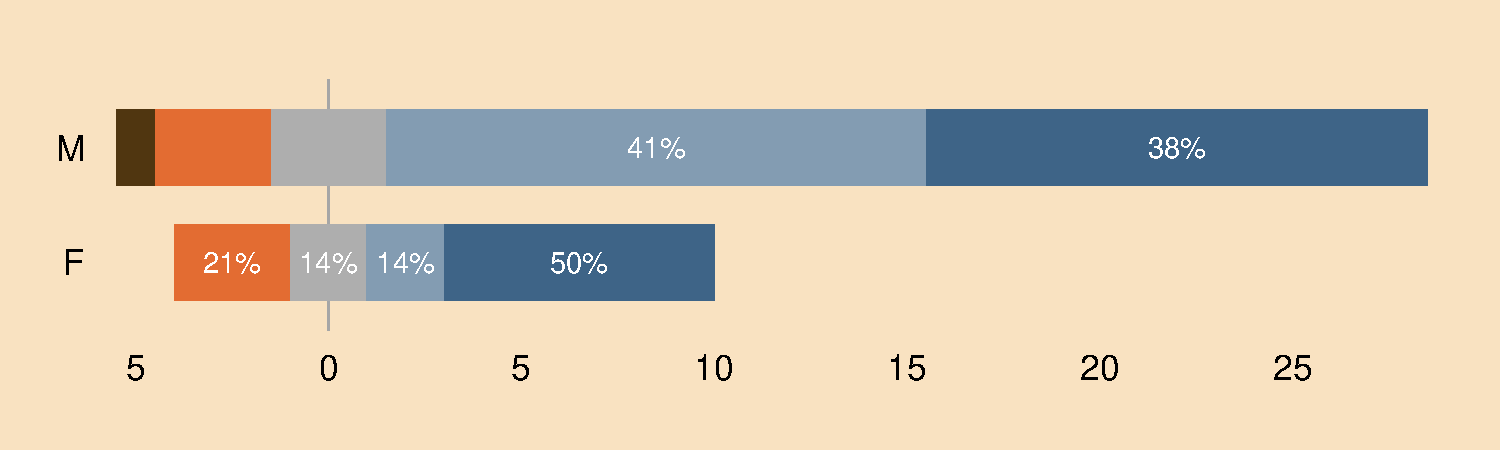
\includegraphics[align=t,trim={0 0 0 15mm},clip,width=11cm]{fig/culture/paolo3.pdf}\\

\hdashline

I feel reporting unfair treatment could affect my career & 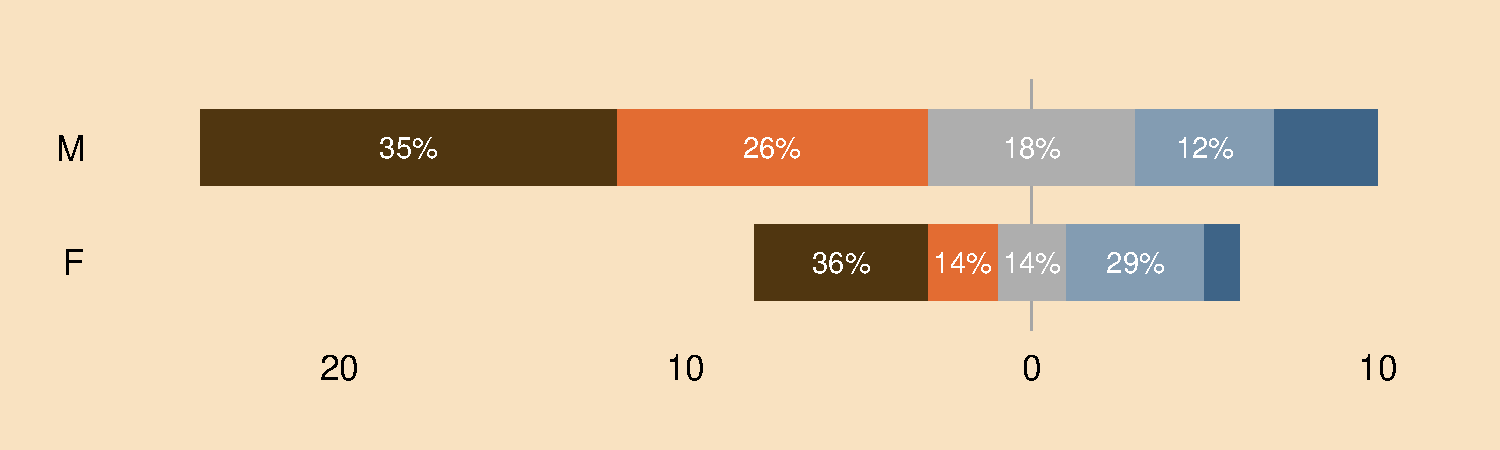
\includegraphics[align=t,trim={0 0 0 15mm},clip,width=11cm]{fig/culture/paolo4.pdf}\\

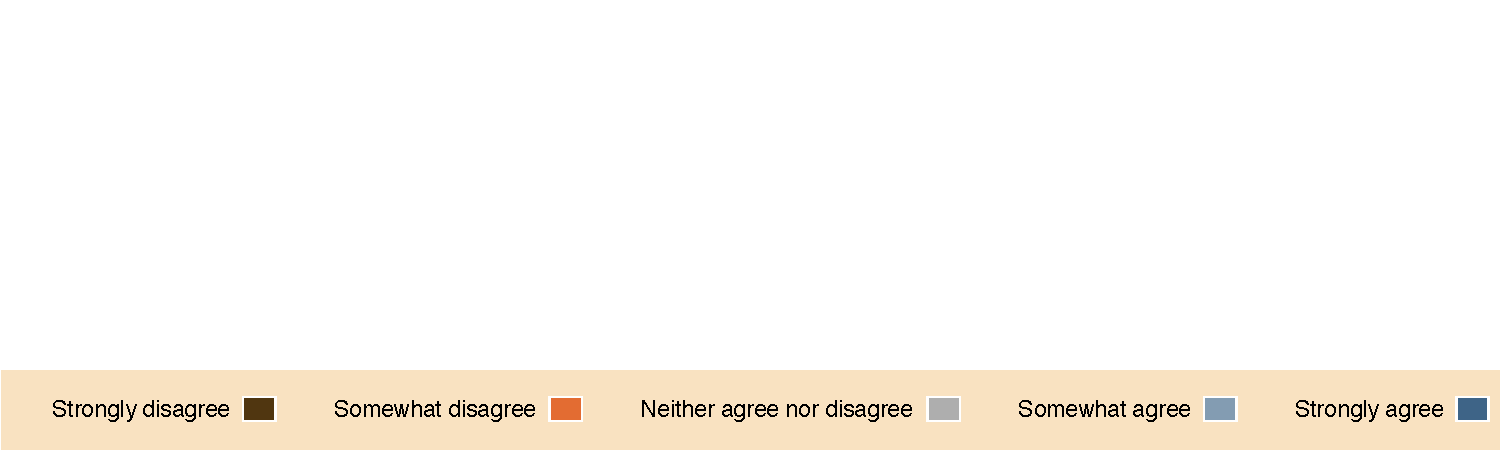
\includegraphics[trim={6mm 0 0 0},clip,width=14.5cm]{fig/legend5col.pdf}\\
\end{tabular}
\end{figbox}
